\scanpage{59}
les \uline{op. diff.} de $M$ dans $N$ (rel à $S$),

Alors, on trouve encore un foncteur en $M$, mais \deleted{tout} non à valeurs dans les $P^i$-Modules, mais \inserted{\figure{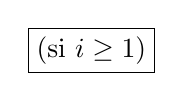
\begin{tikzpicture}
\node[draw,inner sep=3pt] {(si $i\geq1$)};
\end{tikzpicture}}}
seulement dans les $P^{i-1}$-Modules, où on considère $P^i[M]$ comme $P^{i-1}$-Module par \uline{restriction des scalaires} à l'aide de $\alpha^{i-1}:P^{i-1}\longrightarrow P^i$.
\inserted{(On le note alors $Q^{i-1}[M]$) \textcircled{$*$}}
En particulier, $Q^0[M]$ est \deleted{\unsure{le}} un foncteur en
$M\in\operatorname{Ob}\operatorname{Mod}(X/S)$
\inserted{[Modules sur $\mathcal{O}_X$, avec comme hom les op. diff. \deleted{d'ordre} rel. à $S$]},
à valeurs dans les pro-$\mathcal{O}_X$-Modules.
\margin{et qu'on utilise comme morphismes de \deleted{\unsure{type}} $\mathbb{N}$-pro-objets ceux de Artin--Riesz
[\unsure{ce qui revient à ne considérer} que des op. diff. de degré borné, --- qui est autom. si $X$ qu. cpt].}

\deleted{[$P^0[M]=M$ \deleted{\unsure{est}} \unsure{doit} être considéré comme un foncteur à valeurs dans $\operatorname{Ab}(X)$]}

Notons que l'hom $\unsure{\alpha^\bullet|\alpha^*}:P^*\mathbin{-}(SP)^*=Q^*$ permet de considérer $Q^*$ comme \deleted{\unsure{module}} \inserted{algèbre} \deleted{\unsure{pro}} cosimplicial sur l'\deleted{\unsure{anneau}} cosimplicial $P^*$, et que les opérations extrêmes droites

\margin{\figure{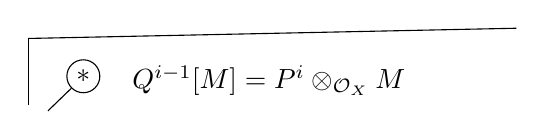
\begin{tikzpicture}
\draw (0,0.7)--(0,-0.15);
\draw (0,0.7)--(6.2,0.83);
\node[draw,circle,inner sep=1.8pt] (star) at (0.7,0.22) {$*$};
\draw (star.south west)--(0.25,-0.22);
\node[anchor=west] at (1.2,0.17) {$Q^{i-1}[M]=P^i\otimes_{\mathcal{O}_X}M$};
\end{tikzpicture}}}
\margin{58}
